
% LaTeX Beamer file automatically generated from DocOnce
% https://github.com/doconce/doconce

%-------------------- begin beamer-specific preamble ----------------------

\documentclass{beamer}

\usetheme{red_plain}
\usecolortheme{default}

% turn off the almost invisible, yet disturbing, navigation symbols:
\setbeamertemplate{navigation symbols}{}

% Examples on customization:
%\usecolortheme[named=RawSienna]{structure}
%\usetheme[height=7mm]{Rochester}
%\setbeamerfont{frametitle}{family=\rmfamily,shape=\itshape}
%\setbeamertemplate{items}[ball]
%\setbeamertemplate{blocks}[rounded][shadow=true]
%\useoutertheme{infolines}
%
%\usefonttheme{}
%\useinntertheme{}
%
%\setbeameroption{show notes}
%\setbeameroption{show notes on second screen=right}

% fine for B/W printing:
%\usecolortheme{seahorse}

\usepackage{pgf}
\usepackage{graphicx}
\usepackage{epsfig}
\usepackage{relsize}

\usepackage{fancybox}  % make sure fancybox is loaded before fancyvrb

\usepackage{fancyvrb}
%\usepackage{minted} % requires pygments and latex -shell-escape filename
%\usepackage{anslistings}
%\usepackage{listingsutf8}

\usepackage{amsmath,amssymb,bm}
%\usepackage[latin1]{inputenc}
\usepackage[T1]{fontenc}
\usepackage[utf8]{inputenc}
\usepackage{colortbl}
\usepackage[english]{babel}
\usepackage{tikz}
\usepackage{framed}
% Use some nice templates
\beamertemplatetransparentcovereddynamic

% --- begin table of contents based on sections ---
% Delete this, if you do not want the table of contents to pop up at
% the beginning of each section:
% (Only section headings can enter the table of contents in Beamer
% slides generated from DocOnce source, while subsections are used
% for the title in ordinary slides.)
\AtBeginSection[]
{
  \begin{frame}<beamer>[plain]
  \frametitle{}
  %\frametitle{Outline}
  \tableofcontents[currentsection]
  \end{frame}
}
% --- end table of contents based on sections ---

% If you wish to uncover everything in a step-wise fashion, uncomment
% the following command:

%\beamerdefaultoverlayspecification{<+->}

\newcommand{\shortinlinecomment}[3]{\note{\textbf{#1}: #2}}
\newcommand{\longinlinecomment}[3]{\shortinlinecomment{#1}{#2}{#3}}

\definecolor{linkcolor}{rgb}{0,0,0.4}
\hypersetup{
    colorlinks=true,
    linkcolor=linkcolor,
    urlcolor=linkcolor,
    pdfmenubar=true,
    pdftoolbar=true,
    bookmarksdepth=3
    }
\setlength{\parskip}{0pt}  % {1em}

\newenvironment{doconceexercise}{}{}
\newcounter{doconceexercisecounter}
\newenvironment{doconce:movie}{}{}
\newcounter{doconce:movie:counter}

\newcommand{\subex}[1]{\noindent\textbf{#1}}  % for subexercises: a), b), etc

%-------------------- end beamer-specific preamble ----------------------

% Add user's preamble




% insert custom LaTeX commands...

\raggedbottom
\makeindex

%-------------------- end preamble ----------------------

\begin{document}

% matching end for #ifdef PREAMBLE

\newcommand{\exercisesection}[1]{\subsection*{#1}}



% ------------------- main content ----------------------



% ----------------- title -------------------------

\title{Machine learning approaches for quantum mechanical problems}

% ----------------- author(s) -------------------------

\author{Morten Hjorth-Jensen\inst{1,2}}
\institute{Department of Physics and Center for Computing in Science Education, University of Oslo, Norway\inst{1}
\and
Department of Physics and Astronomy and Facility for Rare Isotope Beams, Michigan State University, East Lansing, Michigan, USA\inst{2}}
% ----------------- end author(s) -------------------------

\date{PhysML workshop, Oslo, Norway, May 14-16, 2024
% <optional titlepage figure>
% <optional copyright>
}

\begin{frame}[plain,fragile]
\titlepage
\end{frame}

\begin{frame}[plain,fragile]
\frametitle{What is this talk about?}

\begin{block}{}

The main aim is to give you a short and hopefully pedestrian
introduction to machine learning methods for solving quantum
mechanical many-body problems.

The first part has an emphasis on both generative and discriminative
methods while the second part of the talk introduces a new method
dubbed \textbf{Parametric Matrix Models}, see
\href{{https://arxiv.org/abs/2401.11694}}{\nolinkurl{https://arxiv.org/abs/2401.11694}}.
\end{block}

\begin{block}{}
These slides and more at \href{{https://github.com/mhjensenseminars/MachineLearningTalk/tree/master/doc/pub/sintefml}}{\nolinkurl{https://github.com/mhjensenseminars/MachineLearningTalk/tree/master/doc/pub/sintefml}}
\end{block}
\end{frame}

\begin{frame}[plain,fragile]
\frametitle{Thanks to many}

Jane Kim (MSU/Ohio U), Julie Butler (MSU/Mt Union), Patrick Cook (MSU), Danny Jammooa (MSU), Daniel Bazin (MSU), Dean Lee (MSU), Daniel Lee (Cornell), Even Nordhagen (UiO), Robert Solli (UiO, Expert Analytics), Bryce Fore (ANL), Alessandro Lovato (ANL), Stefano Gandolfi (LANL), Francesco Pederiva (UniTN), and Giuseppe Carleo (EPFL).
\end{frame}

\begin{frame}[plain,fragile]
\frametitle{And sponsors}

\begin{enumerate}
\item National Science Foundation, USA (various grants)

\item Department of Energy, USA (various grants)

\item Research Council of Norway (various grants) and my employers University of Oslo and Michigan State University
\end{enumerate}

\noindent
\end{frame}

\begin{frame}[plain,fragile]
\frametitle{Background}

\begin{block}{}
\begin{enumerate}
\item I have my training and research in traditional many-body theories and have studied and coded almost all, FCI, mean-field methods, Coupled Cluster theories, Green's function approaches, many-body perturbation theories, Monte Carlo methods and also molecular dynamics. Time independent and time-dependent theories

\item Central keywords: Effective degrees of freedom and dimensionality reduction

\item Last 6-8 years  focus on quantum computing and machine learning

\item Developed many courses (regular and intensive) ones on many-body physics, computational physics, machine learning and quantum computing, see \href{{https://github.com/mhjensen}}{\nolinkurl{https://github.com/mhjensen}}
\end{enumerate}

\noindent
\end{block}
\end{frame}

\begin{frame}[plain,fragile]
\frametitle{Selected references}

\begin{block}{}
\begin{itemize}
\item A high-bias, low-variance introduction to Machine Learning for physicists, Mehta et al., Physics Reports \textbf{810}, 1 (2019), \href{{https://www.sciencedirect.com/science/article/pii/S0370157319300766?via%3Dihub}}{\nolinkurl{https://www.sciencedirect.com/science/article/pii/S0370157319300766?via\%3Dihub}}.

\item Machine Learning and the Physical Sciences by Carleo et al., Reviews of Modern Physics \textbf{91}, 045002 (2019), \href{{https://link.aps.org/doi/10.1103/RevModPhys.91.045002}}{\nolinkurl{https://link.aps.org/doi/10.1103/RevModPhys.91.045002}}

\item Artificial Intelligence and Machine Learning in Nuclear Physics, Amber Boehnlein et al., Reviews Modern of Physics \textbf{94}, 031003 (2022), \href{{https://journals.aps.org/rmp/abstract/10.1103/RevModPhys.94.031003}}{\nolinkurl{https://journals.aps.org/rmp/abstract/10.1103/RevModPhys.94.031003}} 

\item Dilute neutron star matter from neural-network quantum states by Fore et al, Physical Review Research \textbf{5}, 033062 (2023), \href{{https://journals.aps.org/prresearch/pdf/10.1103/PhysRevResearch.5.033062}}{\nolinkurl{https://journals.aps.org/prresearch/pdf/10.1103/PhysRevResearch.5.033062}}
\end{itemize}

\noindent
\end{block}
\end{frame}

\begin{frame}[plain,fragile]
\frametitle{Selected references}

\begin{block}{}
\begin{itemize}
\item Neural-network quantum states for ultra-cold Fermi gases, Jane Kim et al, Nature Communications Physics \textbf{7}, 148 (2024), \href{{https://www.nature.com/articles/s42005-024-01613-w}}{\nolinkurl{https://www.nature.com/articles/s42005-024-01613-w}}

\item Message-Passing Neural Quantum States for the Homogeneous Electron Gas, Gabriel Pescia, Jane Kim et al.~arXiv.2305.07240,":"https://doi.org/10.48550/arXiv.2305.07240"

\item Parametric Matrix Models, Patrick Cook, Danny Jammooa, MHJ, Dean Lee and Daniel Lee, \href{{https://arxiv.org/abs/2401.11694}}{\nolinkurl{https://arxiv.org/abs/2401.11694}}. 
\end{itemize}

\noindent
\end{block}
\end{frame}

\begin{frame}[plain,fragile]
\frametitle{Extrapolations and model interpretability}

When you hear phrases like \textbf{predictions and estimations} and
\textbf{correlations and causations}, what do you think of?

May be you think
of the difference between classifying new data points and generating
new data points.

Or perhaps you consider that correlations represent some kind of symmetric statements like
if $A$ is correlated with $B$, then $B$ is correlated with
$A$. Causation on the other hand is directional, that is if $A$ causes $B$, $B$ does not
necessarily cause $A$.
\end{frame}

\begin{frame}[plain,fragile]
\frametitle{Generative and discriminative models}

\begin{block}{}
\begin{enumerate}
\item Balance between tractability and flexibility

\item We want to extract information about correlations, to make predictions, quantify uncertainties and express causality

\item How do we represent reliably our effective degrees of freedom?
\end{enumerate}

\noindent
\end{block}
\end{frame}

\begin{frame}[plain,fragile]
\frametitle{Example of generative modeling, \href{{https://www.oreilly.com/library/view/generative-deep-learning/9781098134174/ch01.html}}{taken from Generative Deep Learning by David Foster}}

\vspace{6mm}

% inline figure
\centerline{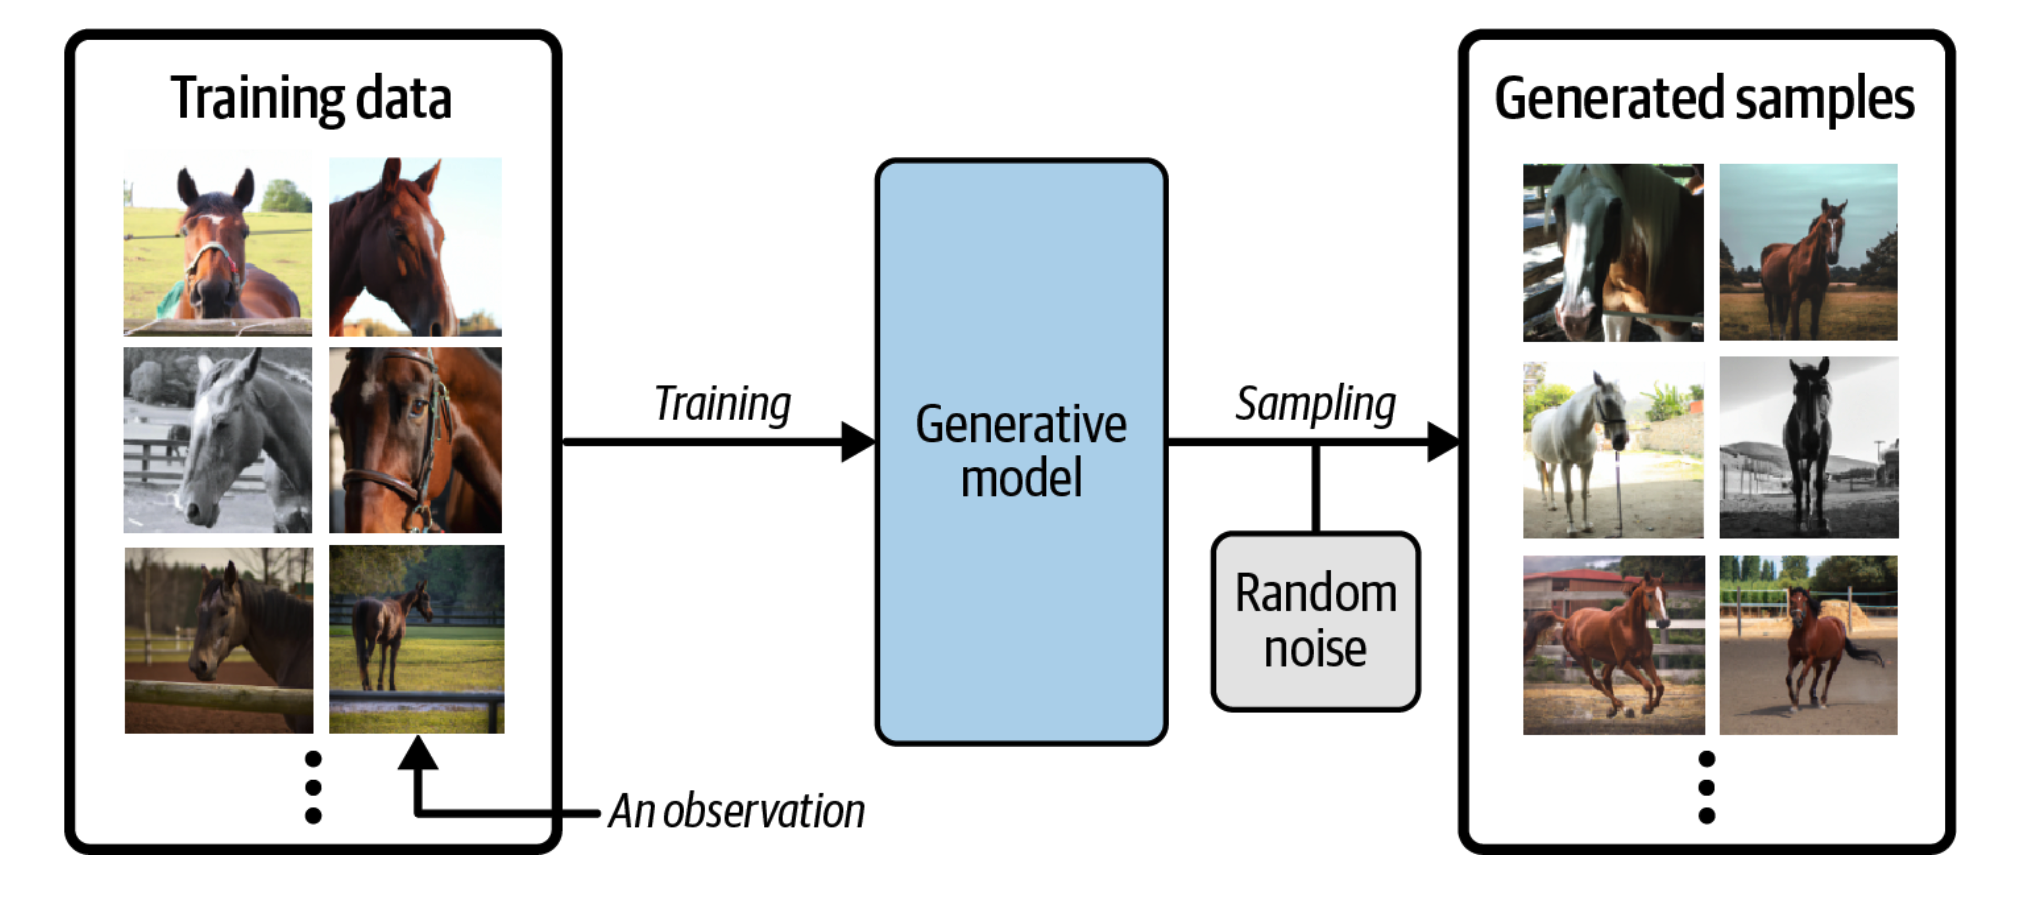
\includegraphics[width=1.0\linewidth]{figures/generativelearning.png}}

\vspace{6mm}
\end{frame}

\begin{frame}[plain,fragile]
\frametitle{Example of discriminative modeling, \href{{https://www.oreilly.com/library/view/generative-deep-learning/9781098134174/ch01.html}}{taken from Generative Deeep Learning by David Foster}}

\vspace{6mm}

% inline figure
\centerline{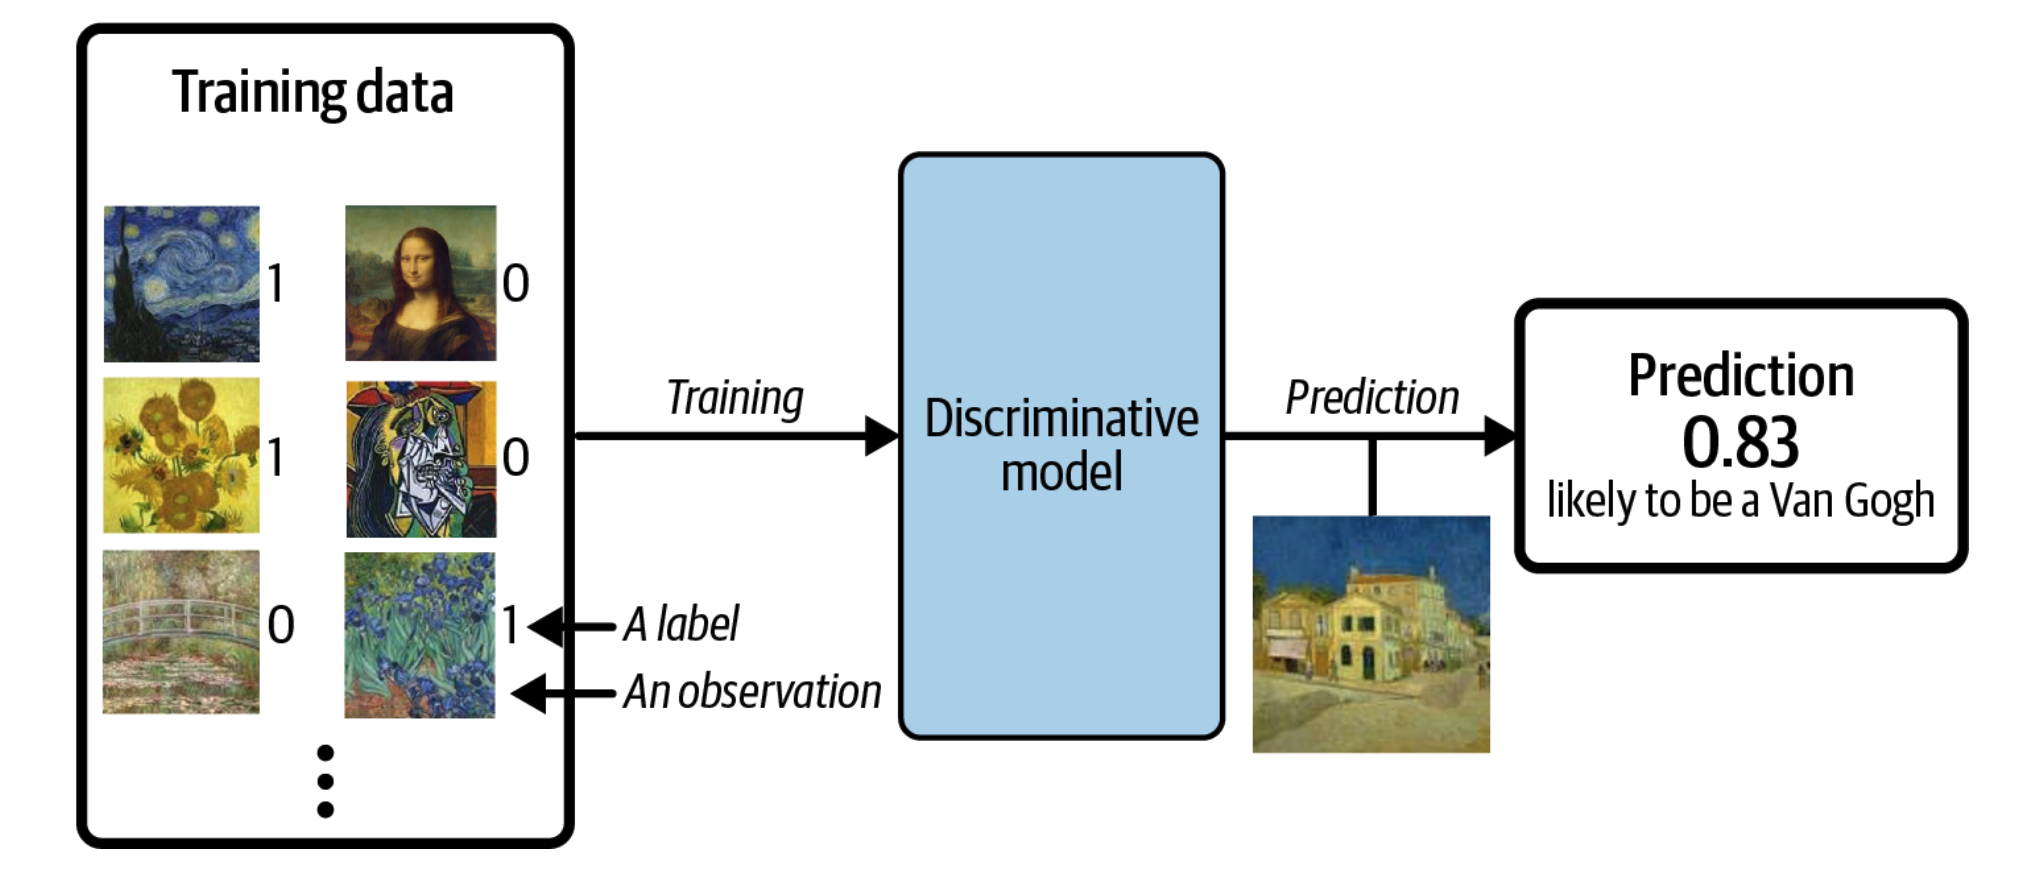
\includegraphics[width=1.0\linewidth]{figures/standarddeeplearning.png}}

\vspace{6mm}
\end{frame}

\begin{frame}[plain,fragile]
\frametitle{Machine learning. A simple perspective on the interface between ML and Physics}

\vspace{6mm}

% inline figure
\centerline{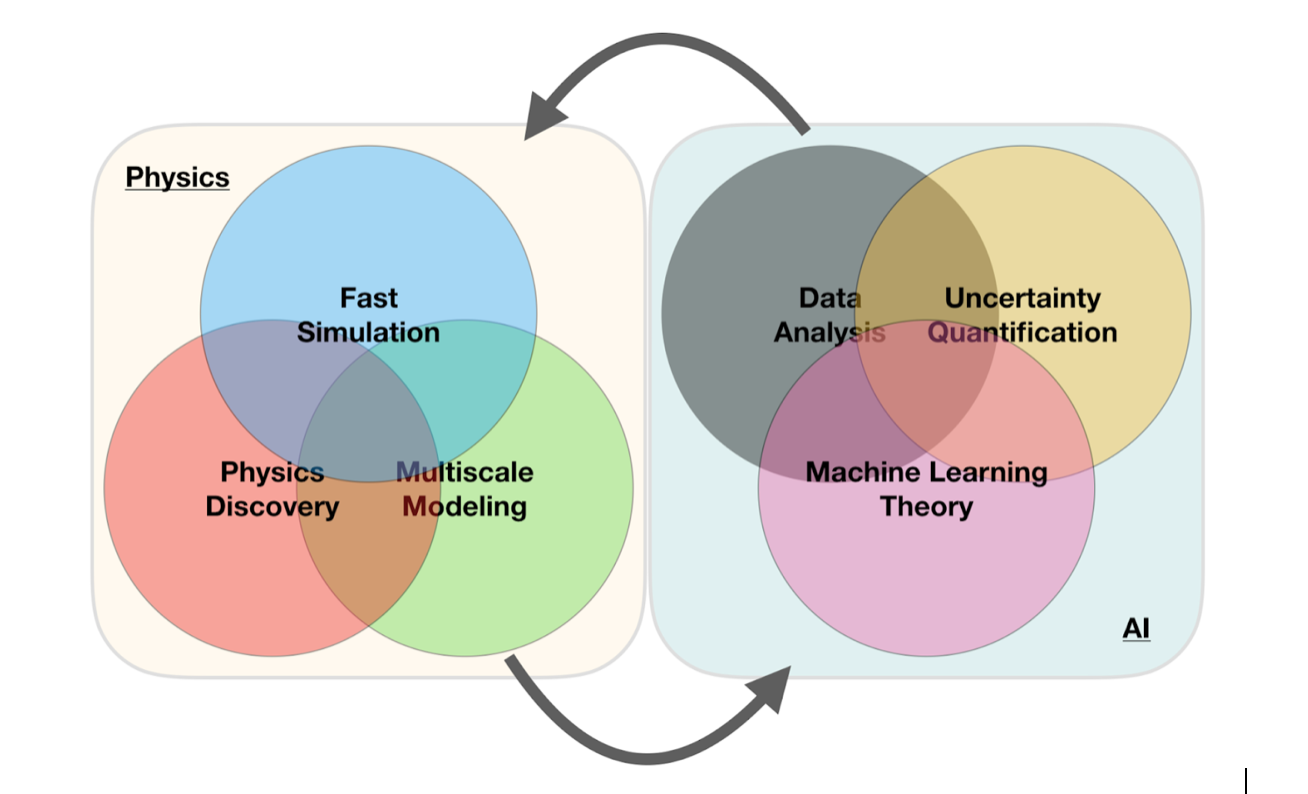
\includegraphics[width=1.0\linewidth]{figures/mlimage.png}}

\vspace{6mm}
\end{frame}

\begin{frame}[plain,fragile]
\frametitle{Many-body physics, Quantum Monte Carlo and deep learning}

\begin{block}{}
Given a hamiltonian $H$ and a trial wave function $\Psi_T$, the variational principle states that the expectation value of $\langle H \rangle$, defined through 
\[
   \langle E \rangle =
   \frac{\int d\bm{R}\Psi^{\ast}_T(\bm{R})H(\bm{R})\Psi_T(\bm{R})}
        {\int d\bm{R}\Psi^{\ast}_T(\bm{R})\Psi_T(\bm{R})},
\]
is an upper bound to the ground state energy $E_0$ of the hamiltonian $H$, that is 
\[
    E_0 \le \langle E \rangle.
\]
In general, the integrals involved in the calculation of various  expectation values  are multi-dimensional ones. Traditional integration methods such as the Gauss-Legendre will not be adequate for say the  computation of the energy of a many-body system.  \textbf{Basic philosophy: Let a neural network find the optimal wave function}
\end{block}
\end{frame}

\begin{frame}[plain,fragile]
\frametitle{Quantum Monte Carlo Motivation}

\begin{block}{Basic steps }
Choose a trial wave function
$\psi_T(\bm{R})$.
\[
   P(\bm{R},\bm{\alpha})= \frac{\left|\psi_T(\bm{R},\bm{\alpha})\right|^2}{\int \left|\psi_T(\bm{R},\bm{\alpha})\right|^2d\bm{R}}.
\]
This is our model, or likelihood/probability distribution function  (PDF). It depends on some variational parameters $\bm{\alpha}$.
The approximation to the expectation value of the Hamiltonian is now 
\[
   \langle E[\bm{\alpha}] \rangle = 
   \frac{\int d\bm{R}\Psi^{\ast}_T(\bm{R},\bm{\alpha})H(\bm{R})\Psi_T(\bm{R},\bm{\alpha})}
        {\int d\bm{R}\Psi^{\ast}_T(\bm{R},\bm{\alpha})\Psi_T(\bm{R},\bm{\alpha})}.
\]
\end{block}
\end{frame}

\begin{frame}[plain,fragile]
\frametitle{Quantum Monte Carlo Motivation}

\begin{block}{Define a new quantity }
\[
   E_L(\bm{R},\bm{\alpha})=\frac{1}{\psi_T(\bm{R},\bm{\alpha})}H\psi_T(\bm{R},\bm{\alpha}),
\]
called the local energy, which, together with our trial PDF yields
\[
  \langle E[\bm{\alpha}] \rangle=\int P(\bm{R})E_L(\bm{R},\bm{\alpha}) d\bm{R}\approx \frac{1}{N}\sum_{i=1}^NE_L(\bm{R_i},\bm{\alpha})
\]
with $N$ being the number of Monte Carlo samples.
\end{block}
\end{frame}

\begin{frame}[plain,fragile]
\frametitle{Energy derivatives}

\begin{block}{}
The local energy as function of the variational parameters defines now our \textbf{objective/cost} function.

To find the derivatives of the local energy expectation value as function of the variational parameters, we can use the chain rule and the hermiticity of the Hamiltonian.  

Let us define (with the notation $\langle E[\bm{\alpha}]\rangle =\langle  E_L\rangle$)
\[
\bar{E}_{\alpha_i}=\frac{d\langle  E_L\rangle}{d\alpha_i},
\]
as the derivative of the energy with respect to the variational parameter $\alpha_i$
We define also the derivative of the trial function (skipping the subindex $T$) as 
\[
\bar{\Psi}_{i}=\frac{d\Psi}{d\alpha_i}.
\]
\end{block}
\end{frame}

\begin{frame}[plain,fragile]
\frametitle{Derivatives of the local energy}

\begin{block}{}
The elements of the gradient of the local energy are 
\[
\bar{E}_{i}= 2\left( \langle \frac{\bar{\Psi}_{i}}{\Psi}E_L\rangle -\langle \frac{\bar{\Psi}_{i}}{\Psi}\rangle\langle E_L \rangle\right).
\]
From a computational point of view it means that you need to compute the expectation values of 
\[
\langle \frac{\bar{\Psi}_{i}}{\Psi}E_L\rangle,
\]
and
\[
\langle \frac{\bar{\Psi}_{i}}{\Psi}\rangle\langle E_L\rangle
\]
These integrals are evaluted using MC intergration (with all its possible error sources). Use methods like stochastic gradient or other minimization methods to find the optimal parameters.
\end{block}
\end{frame}

\begin{frame}[plain,fragile]
\frametitle{Why Feed Forward Neural Networks (FFNN)?}

According to the \emph{Universal approximation theorem}, a feed-forward
neural network with just a single hidden layer containing a finite
number of neurons can approximate a continuous multidimensional
function to arbitrary accuracy, assuming the activation function for
the hidden layer is a \textbf{non-constant, bounded and
monotonically-increasing continuous function}.
\end{frame}

\begin{frame}[plain,fragile]
\frametitle{Universal approximation theorem}

The universal approximation theorem plays a central role in deep
learning.  \href{{https://link.springer.com/article/10.1007/BF02551274}}{Cybenko (1989)} showed
the following:

\begin{block}{}
Let $\sigma$ be any continuous sigmoidal function such that
\[
\sigma(z) = \left\{\begin{array}{cc} 1 & z\rightarrow \infty\\ 0 & z \rightarrow -\infty \end{array}\right.
\]
Given a continuous and deterministic function $F(\bm{x})$ on the unit
cube in $d$-dimensions $F\in [0,1]^d$, $x\in [0,1]^d$ and a parameter
$\epsilon >0$, there is a one-layer (hidden) neural network
$f(\bm{x};\bm{\Theta})$ with $\bm{\Theta}=(\bm{W},\bm{b})$ and $\bm{W}\in
\mathbb{R}^{m\times n}$ and $\bm{b}\in \mathbb{R}^{n}$, for which
\[
\vert F(\bm{x})-f(\bm{x};\bm{\Theta})\vert < \epsilon \hspace{0.1cm} \forall \bm{x}\in[0,1]^d.
\]

\end{block}
\end{frame}

\begin{frame}[plain,fragile]
\frametitle{The approximation theorem in words}

\textbf{Any continuous function $y=F(\bm{x})$ supported on the unit cube in
$d$-dimensions can be approximated by a one-layer sigmoidal network to
arbitrary accuracy.}

\href{{https://www.sciencedirect.com/science/article/abs/pii/089360809190009T}}{Hornik (1991)} extended the theorem by letting any non-constant, bounded activation function to be included using that the expectation value
\[
\mathbb{E}[\vert F(\bm{x})\vert^2] =\int_{\bm{x}\in D} \vert F(\bm{x})\vert^2p(\bm{x})d\bm{x} < \infty.
\]
Then we have
\[
\mathbb{E}[\vert F(\bm{x})-f(\bm{x};\bm{\Theta})\vert^2] =\int_{\bm{x}\in D} \vert F(\bm{x})-f(\bm{x};\bm{\Theta})\vert^2p(\bm{x})d\bm{x} < \epsilon.
\]
\end{frame}

\begin{frame}[plain,fragile]
\frametitle{More on the general approximation theorem}

None of the proofs give any insight into the relation between the
number of of hidden layers and nodes and the approximation error
$\epsilon$, nor the magnitudes of $\bm{W}$ and $\bm{b}$.

Neural networks (NNs) have what we may call a kind of universality no matter what function we want to compute.

\begin{block}{}
It does not mean that an NN can be used to exactly compute any function. Rather, we get an approximation that is as good as we want. 
\end{block}
\end{frame}

\begin{frame}[plain,fragile]
\frametitle{Class of functions we can approximate}

\begin{block}{}
The class of functions that can be approximated are the continuous ones.
If the function $F(\bm{x})$ is discontinuous, it won't in general be possible to approximate it. However, an NN may still give an approximation even if we fail in some points.
\end{block}
\end{frame}

\begin{frame}[plain,fragile]
\frametitle{Illustration of a single perceptron model and an FFNN}

\begin{figure}[!ht]  % 
  \centerline{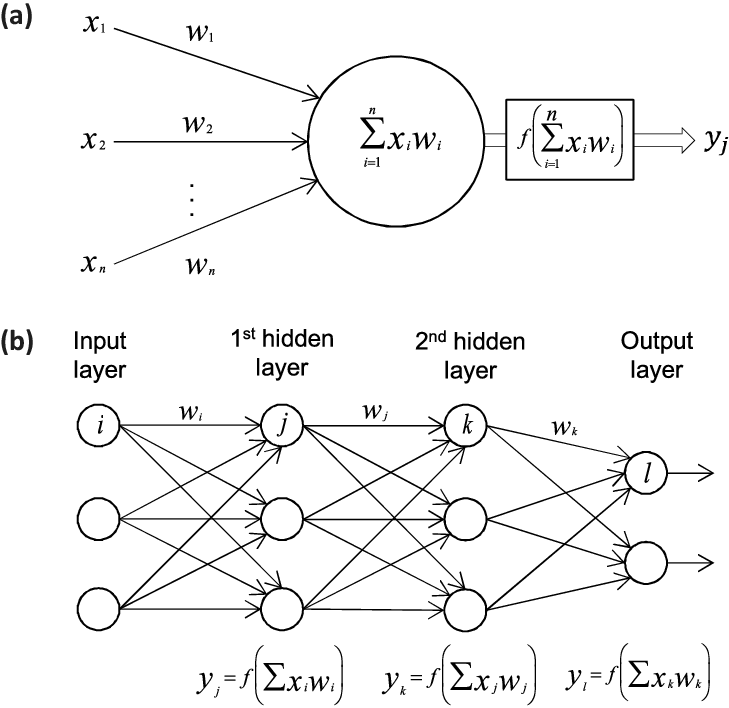
\includegraphics[width=0.7\linewidth]{figures/nns.png}}
  \caption{
  In a) we show a single perceptron model while in b) we dispay a network with two  hidden layers, an input layer and an output layer.
  }
\end{figure}
%\clearpage % flush figures
\end{frame}

\begin{frame}[plain,fragile]
\frametitle{Monte Carlo methods and Neural Networks}

\href{{https://www.sciencedirect.com/science/article/pii/S0370269320305463?via%3Dihub}}{Machine Learning and the Deuteron by Kebble and Rios} and
\href{{https://journals.aps.org/prl/abstract/10.1103/PhysRevLett.127.022502}}{Variational Monte Carlo calculations of $A\le 4$ nuclei with an artificial neural-network correlator ansatz by Adams et al.}

\textbf{Adams et al}:

\begin{align}
H_{LO} &=-\sum_i \frac{{\vec{\nabla}_i^2}}{2m_N}
+\sum_{i<j} {\left(C_1  + C_2\, \vec{\sigma_i}\cdot\vec{\sigma_j}\right)
e^{-r_{ij}^2\Lambda^2 / 4 }}
\nonumber\\
&+D_0 \sum_{i<j<k} \sum_{\text{cyc}}
{e^{-\left(r_{ik}^2+r_{ij}^2\right)\Lambda^2/4}}\,,
\end{align}

where $m_N$ is the mass of the nucleon, $\vec{\sigma_i}$ is the Pauli
matrix acting on nucleon $i$, and $\sum_{\text{cyc}}$ stands for the
cyclic permutation of $i$, $j$, and $k$. The low-energy constants
$C_1$ and $C_2$ are fit to the deuteron binding energy and to the
neutron-neutron scattering length
\end{frame}

\begin{frame}[plain,fragile]
\frametitle{Deep learning neural networks, \href{{https://journals.aps.org/prl/abstract/10.1103/PhysRevLett.127.022502}}{Variational Monte Carlo calculations of $A\le 4$ nuclei with an artificial neural-network correlator ansatz by Adams et al.}}

An appealing feature of the neural network ansatz is that it is more general than the more conventional product of two-
and three-body spin-independent Jastrow functions
\begin{align}
|\Psi_V^J \rangle = \prod_{i<j<k} \Big( 1-\sum_{\text{cyc}} u(r_{ij}) u(r_{jk})\Big) \prod_{i<j} f(r_{ij}) | \Phi\rangle\,,
\end{align}
which is commonly used for nuclear Hamiltonians that do not contain tensor and spin-orbit terms.
The above function is replaced by a multi-layer Neural Network.
\end{frame}

\begin{frame}[plain,fragile]
\frametitle{\href{{https://journals.aps.org/prresearch/pdf/10.1103/PhysRevResearch.5.033062}}{Dilute neutron star matter from neural-network quantum states by Fore et al, Physical Review Research 5, 033062 (2023)} at density $\rho=0.04$ fm$^{-3}$}

\begin{block}{}

\vspace{6mm}

% inline figure
\centerline{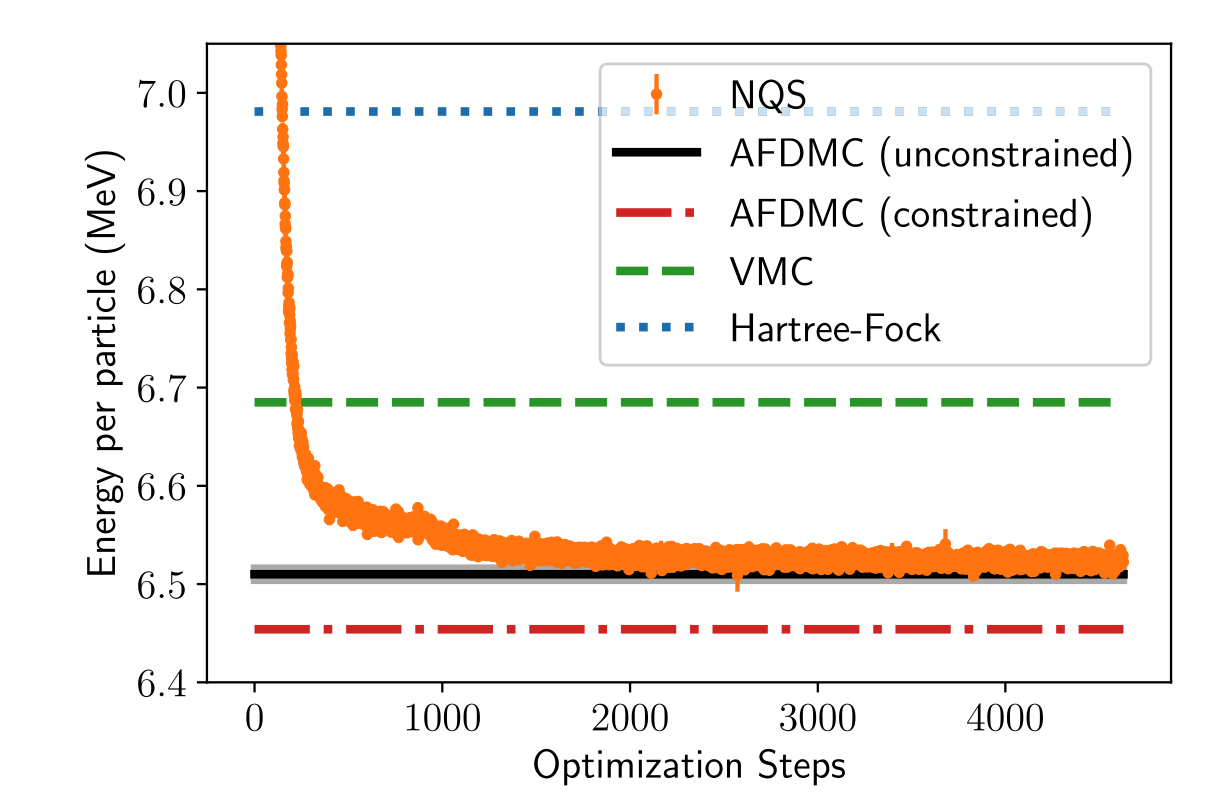
\includegraphics[width=0.9\linewidth]{figures/nmatter.png}}

\vspace{6mm}

\end{block}
\end{frame}

\begin{frame}[plain,fragile]
\frametitle{Pairing and Spin-singlet and triplet two-body distribution functions at $\rho=0.01$ fm$^{-3}$}

\begin{block}{}

\vspace{6mm}

% inline figure
\centerline{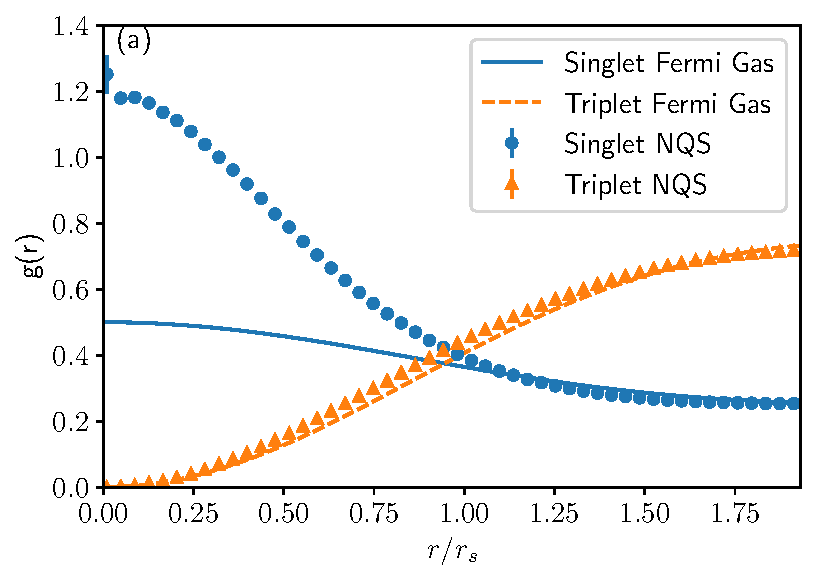
\includegraphics[width=0.9\linewidth]{figures/01_tbd.pdf}}

\vspace{6mm}

\end{block}
\end{frame}

\begin{frame}[plain,fragile]
\frametitle{Pairing and Spin-singlet and triplet two-body distribution functions at $\rho=0.04$ fm$^{-3}$}

\begin{block}{}

\vspace{6mm}

% inline figure
\centerline{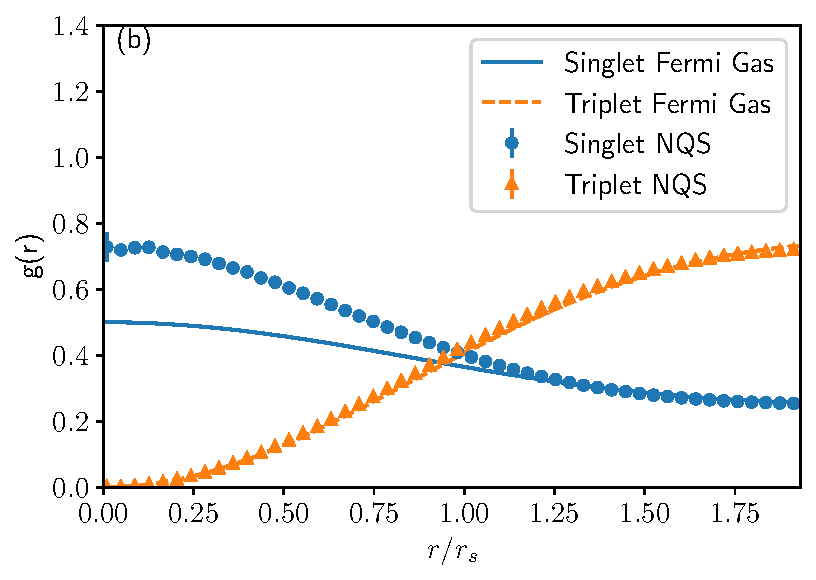
\includegraphics[width=0.9\linewidth]{figures/04_tbd.pdf}}

\vspace{6mm}

\end{block}
\end{frame}

\begin{frame}[plain,fragile]
\frametitle{Pairing and Spin-singlet and triplet two-body distribution functions at $\rho=0.08$ fm$^{-3}$}

\begin{block}{}

\vspace{6mm}

% inline figure
\centerline{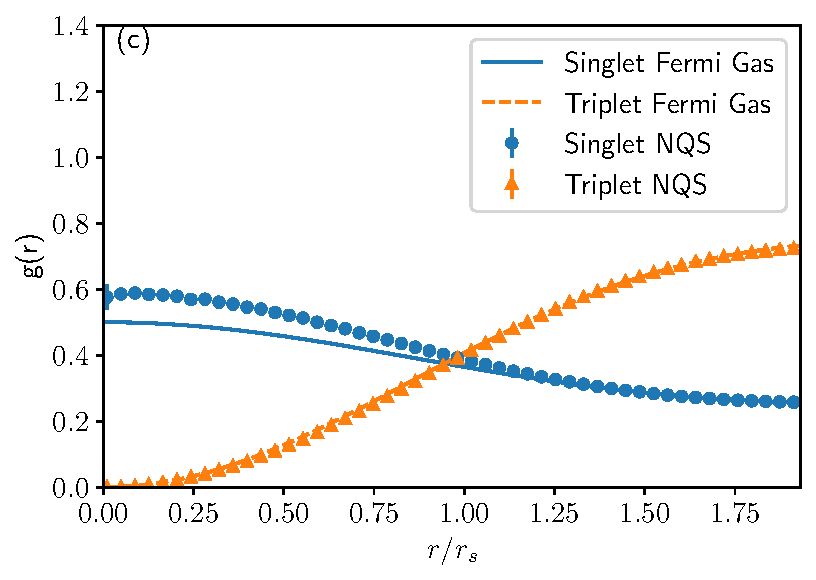
\includegraphics[width=0.9\linewidth]{figures/08_tbd.pdf}}

\vspace{6mm}

\end{block}
\end{frame}

\begin{frame}[plain,fragile]
\frametitle{The electron gas in three dimensions with $N=14$ electrons (Wigner-Seitz radius $r_s=2$ a.u.), \href{{https://doi.org/10.48550/arXiv.2305.07240}}{Gabriel Pescia, Jane Kim et al.~arXiv.2305.07240,}}

\begin{block}{}

\vspace{6mm}

% inline figure
\centerline{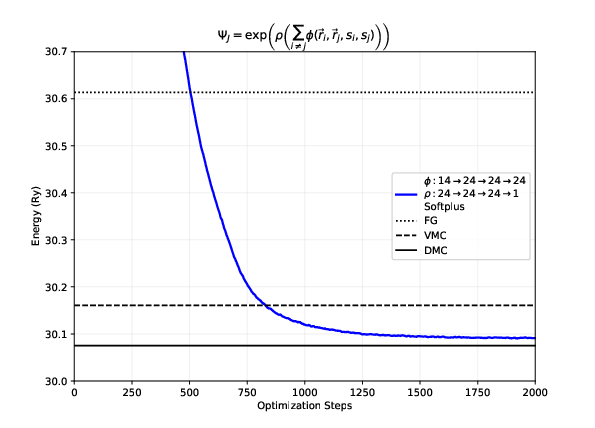
\includegraphics[width=0.9\linewidth]{figures/elgasnew.png}}

\vspace{6mm}

\end{block}
\end{frame}

\begin{frame}[plain,fragile]
\frametitle{Generical approaches to probability models}

We define a probability
\[
p(x_i,h_j;\bm{\Theta}) = \frac{f(x_i,h_j;\bm{\Theta})}{Z(\bm{\Theta})},
\]
where $f(x_i,h_j;\bm{\Theta})$ is a function which we assume is larger or
equal than zero and obeys all properties required for a probability
distribution and $Z(\bm{\Theta})$ is a normalization constant. Inspired by
statistical mechanics, we call it often for the partition function.
It is defined as (assuming that we have discrete probability distributions)
\[
Z(\bm{\Theta})=\sum_{x_i\in \bm{X}}\sum_{h_j\in \bm{H}} f(x_i,h_j;\bm{\Theta}).
\]
\end{frame}

\begin{frame}[plain,fragile]
\frametitle{Marginal and conditional probabilities}

We can in turn define the marginal probabilities
\[
p(x_i;\bm{\Theta}) = \frac{\sum_{h_j\in \bm{H}}f(x_i,h_j;\bm{\Theta})}{Z(\bm{\Theta})},
\]
and 
\[
p(h_i;\bm{\Theta}) = \frac{\sum_{x_i\in \bm{X}}f(x_i,h_j;\bm{\Theta})}{Z(\bm{\Theta})}.
\]
\end{frame}

\begin{frame}[plain,fragile]
\frametitle{Change of notation}

\textbf{Note the change to a vector notation}. A variable like $\bm{x}$
represents now a specific \textbf{configuration}. We can generate an infinity
of such configurations. The final partition function is then the sum
over all such possible configurations, that is

\[
Z(\bm{\Theta})=\sum_{x_i\in \bm{X}}\sum_{h_j\in \bm{H}} f(x_i,h_j;\bm{\Theta}),
\]
changes to
\[
Z(\bm{\Theta})=\sum_{\bm{x}}\sum_{\bm{h}} f(\bm{x},\bm{h};\bm{\Theta}).
\]
If we have a binary set of variable $x_i$ and $h_j$ and $M$ values of $x_i$ and $N$ values of $h_j$ we have in total $2^M$ and $2^N$ possible $\bm{x}$ and $\bm{h}$ configurations, respectively.

We see that even for the modest binary case, we can easily approach a
number of configuration which is not possible to deal with.
\end{frame}

\begin{frame}[plain,fragile]
\frametitle{Optimization problem}

At the end, we are not interested in the probabilities of the hidden variables. The probability we thus want to optimize is 
\[
p(\bm{X};\bm{\Theta})=\prod_{x_i\in \bm{X}}p(x_i;\bm{\Theta})=\prod_{x_i\in \bm{X}}\left(\frac{\sum_{h_j\in \bm{H}}f(x_i,h_j;\bm{\Theta})}{Z(\bm{\Theta})}\right),
\]
which we rewrite as
\[
p(\bm{X};\bm{\Theta})=\frac{1}{Z(\bm{\Theta})}\prod_{x_i\in \bm{X}}\left(\sum_{h_j\in \bm{H}}f(x_i,h_j;\bm{\Theta})\right).
\]
\end{frame}

\begin{frame}[plain,fragile]
\frametitle{Further simplifications}

We simplify further by rewriting it as
\[
p(\bm{X};\bm{\Theta})=\frac{1}{Z(\bm{\Theta})}\prod_{x_i\in \bm{X}}f(x_i;\bm{\Theta}),
\]
where we used $p(x_i;\bm{\Theta}) = \sum_{h_j\in \bm{H}}f(x_i,h_j;\bm{\Theta})$.
The optimization problem is then
\[
{\displaystyle \mathrm{arg} \hspace{0.1cm}\max_{\bm{\bm{\Theta}}\in {\mathbb{R}}^{p}}} \hspace{0.1cm}p(\bm{X};\bm{\Theta}).
\]
\end{frame}

\begin{frame}[plain,fragile]
\frametitle{Optimizing the logarithm instead}

Computing the derivatives with respect to the parameters $\bm{\Theta}$ is
easier (and equivalent) with taking the logarithm of the
probability. We will thus optimize
\[
{\displaystyle \mathrm{arg} \hspace{0.1cm}\max_{\bm{\bm{\Theta}}\in {\mathbb{R}}^{p}}} \hspace{0.1cm}\log{p(\bm{X};\bm{\Theta})},
\]
which leads to
\[
\nabla_{\bm{\Theta}}\log{p(\bm{X};\bm{\Theta})}=0.
\]
\end{frame}

\begin{frame}[plain,fragile]
\frametitle{Expression for the gradients}

This leads to the following equation
\[
\nabla_{\bm{\Theta}}\log{p(\bm{X};\bm{\Theta})}=\nabla_{\bm{\Theta}}\left(\sum_{x_i\in \bm{X}}\log{f(x_i;\bm{\Theta})}\right)-\nabla_{\bm{\Theta}}\log{Z(\bm{\Theta})}=0.
\]

The first term is called the positive phase and we assume that we have a model for the function $f$ from which we can sample values. Below we will develop an explicit model for this.
The second term is called the negative phase and is the one which leads to more difficulties.
\end{frame}

\begin{frame}[plain,fragile]
\frametitle{The derivative of the partition function}

The partition function, defined above as
\[
Z(\bm{\Theta})=\sum_{x_i\in \bm{X}}\sum_{h_j\in \bm{H}} f(x_i,h_j;\bm{\Theta}),
\]
is in general the most problematic term. In principle both $x$ and $h$ can span large degrees of freedom, if not even infinitely many ones, and computing the partition function itself is often not desirable or even feasible. The above derivative of the partition function can however be written in terms of an expectation value which is in turn evaluated  using Monte Carlo sampling and the theory of Markov chains, popularly shortened to MCMC (or just MC$^2$).
\end{frame}

\begin{frame}[plain,fragile]
\frametitle{Explicit expression for the derivative}

We can rewrite
\[
\nabla_{\bm{\Theta}}\log{Z(\bm{\Theta})}=\frac{\nabla_{\bm{\Theta}}Z(\bm{\Theta})}{Z(\bm{\Theta})},
\]
which reads in more detail
\[
\nabla_{\bm{\Theta}}\log{Z(\bm{\Theta})}=\frac{\nabla_{\bm{\Theta}} \sum_{x_i\in \bm{X}}f(x_i;\bm{\Theta})   }{Z(\bm{\Theta})}.
\]

We can rewrite the function $f$ (we have assumed that is larger or
equal than zero) as $f=\exp{\log{f}}$. We can then rewrite the last
equation as

\[
\nabla_{\bm{\Theta}}\log{Z(\bm{\Theta})}=\frac{ \sum_{x_i\in \bm{X}} \nabla_{\bm{\Theta}}\exp{\log{f(x_i;\bm{\Theta})}}   }{Z(\bm{\Theta})}.
\]
\end{frame}

\begin{frame}[plain,fragile]
\frametitle{Final expression}

Taking the derivative gives us
\[
\nabla_{\bm{\Theta}}\log{Z(\bm{\Theta})}=\frac{ \sum_{x_i\in \bm{X}}f(x_i;\bm{\Theta}) \nabla_{\bm{\Theta}}\log{f(x_i;\bm{\Theta})}   }{Z(\bm{\Theta})}, 
\]
which is the expectation value of $\log{f}$
\[
\nabla_{\bm{\Theta}}\log{Z(\bm{\Theta})}=\sum_{x_i\sim p}p(x_i;\bm{\Theta}) \nabla_{\bm{\Theta}}\log{f(x_i;\bm{\Theta})},
\]
that is
\[
\nabla_{\bm{\Theta}}\log{Z(\bm{\Theta})}=\mathbb{E}(\log{f(x_i;\bm{\Theta})}).
\]

This quantity is evaluated using Monte Carlo sampling, with Gibbs
sampling as the standard sampling rule.
\end{frame}

\begin{frame}[plain,fragile]
\frametitle{Final expression for the gradients}

This leads to the following equation
\[
\nabla_{\bm{\Theta}}\log{p(\bm{X};\bm{\Theta})}=\nabla_{\bm{\Theta}}\left(\sum_{x_i\in \bm{X}}\log{f(x_i;\bm{\Theta})}\right)-\mathbb{E}_{x\sim p}(\log{f(x_i;\bm{\Theta})})=0.
\]
\end{frame}

\begin{frame}[plain,fragile]
\frametitle{Introducing the energy model}

As we will see below, a typical Boltzmann machines employs a probability distribution
\[
p(\bm{x},\bm{h};\bm{\Theta}) = \frac{f(\bm{x},\bm{h};\bm{\Theta})}{Z(\bm{\Theta})},
\]
where $f(\bm{x},\bm{h};\bm{\Theta})$ is given by a so-called energy model. If we assume that the random variables $x_i$ and $h_j$ take binary values only, for example $x_i,h_j=\{0,1\}$, we have a so-called binary-binary model where
\[
f(\bm{x},\bm{h};\bm{\Theta})=-E(\bm{x}, \bm{h};\bm{\Theta}) = \sum_{x_i\in \bm{X}} x_i a_i+\sum_{h_j\in \bm{H}} b_j h_j + \sum_{x_i\in \bm{X},h_j\in\bm{H}} x_i w_{ij} h_j,
\]
where the set of parameters are given by the biases and weights $\bm{\Theta}=\{\bm{a},\bm{b},\bm{W}\}$.
\textbf{Note the vector notation} instead of $x_i$ and $h_j$ for $f$. The vectors $\bm{x}$ and $\bm{h}$ represent a specific instance of stochastic variables $x_i$ and $h_j$. These arrangements of $\bm{x}$ and $\bm{h}$ lead to a specific energy configuration.
\end{frame}

\begin{frame}[plain,fragile]
\frametitle{More compact notation}

With the above definition we can write the probability as
\[
p(\bm{x},\bm{h};\bm{\Theta}) = \frac{\exp{(\bm{a}^T\bm{x}+\bm{b}^T\bm{h}+\bm{x}^T\bm{W}\bm{h})}}{Z(\bm{\Theta})},
\]
where the biases $\bm{a}$ and $\bm{h}$ and the weights defined by the matrix $\bm{W}$ are the parameters we need to optimize.
\end{frame}

\begin{frame}[plain,fragile]
\frametitle{Examples of gradient expressions}

Since the binary-binary energy model is linear in the parameters $a_i$, $b_j$ and
$w_{ij}$, it is easy to see that the derivatives with respect to the
various optimization parameters yield expressions used in the
evaluation of gradients like
\[
\frac{\partial E(\bm{x}, \bm{h};\bm{\Theta})}{\partial w_{ij}}=-x_ih_j,
\]
and
\[
\frac{\partial E(\bm{x}, \bm{h};\bm{\Theta})}{\partial a_i}=-x_i,
\]
and
\[
\frac{\partial E(\bm{x}, \bm{h};\bm{\Theta})}{\partial b_j}=-h_j.
\]
\end{frame}

\begin{frame}[plain,fragile]
\frametitle{Network Elements, the energy function}

The function $E(\bm{x},\bm{h},\bm{\Theta})$ gives the \textbf{energy} of a
configuration (pair of vectors) $(\bm{x}, \bm{h})$. The lower
the energy of a configuration, the higher the probability of it. This
function also depends on the parameters $\bm{a}$, $\bm{b}$ and
$W$. Thus, when we adjust them during the learning procedure, we are
adjusting the energy function to best fit our problem.
\end{frame}

\begin{frame}[plain,fragile]
\frametitle{Defining different types of RBMs}

There are different variants of RBMs, and the differences lie in the types of visible and hidden units we choose as well as in the implementation of the energy function $E(\bm{x},\bm{h},\bm{\Theta})$. The connection between the nodes in the two layers is given by the weights $w_{ij}$. 

\begin{block}{Binary-Binary RBM: }

RBMs were first developed using binary units in both the visible and hidden layer. The corresponding energy function is defined as follows:
\begin{align*}
	E(\bm{x}, \bm{h},\bm{\Theta}) = - \sum_i^M x_i a_i- \sum_j^N b_j h_j - \sum_{i,j}^{M,N} x_i w_{ij} h_j,
\end{align*}
where the binary values taken on by the nodes are most commonly 0 and 1.
\end{block}
\end{frame}

\begin{frame}[plain,fragile]
\frametitle{Gaussian-binary RBM}

Another varient is the RBM where the visible units are Gaussian while the hidden units remain binary:
\begin{align*}
	E(\bm{x}, \bm{h},\bm{\Theta}) = \sum_i^M \frac{(x_i - a_i)^2}{2\sigma_i^2} - \sum_j^N b_j h_j - \sum_{i,j}^{M,N} \frac{x_i w_{ij} h_j}{\sigma_i^2}. 
\end{align*}

This type of RBMs are useful when we model continuous data (i.e., we wish $\bm{x}$ to be continuous). The paramater $\sigma_i^2$ is meant to represent a variance and is foten just set to one.
\end{frame}

\begin{frame}[plain,fragile]
\frametitle{\href{{https://doi.org/10.3389/fphy.2023.1061580}}{Efficient solutions of fermionic systems using artificial neural networks, Nordhagen et al, Frontiers in Physics 11, 2023}}

The Hamiltonian of the quantum dot is given by
\[ \hat{H} = \hat{H}_0 + \hat{V}, 
\]
where $\hat{H}_0$ is the many-body HO Hamiltonian, and $\hat{V}$ is the
inter-electron Coulomb interactions. In dimensionless units,
\[ \hat{V}= \sum_{i < j}^N \frac{1}{r_{ij}},
\]
with $r_{ij}=\sqrt{\mathbf{r}_i^2 - \mathbf{r}_j^2}$.

Separable Hamiltonian with the relative motion part ($r_{ij}=r$)
\[ 
\hat{H}_r=-\nabla^2_r + \frac{1}{4}\omega^2r^2+ \frac{1}{r},
\]
Analytical solutions in two and three dimensions (\href{{https://journals.aps.org/pra/abstract/10.1103/PhysRevA.48.3561}}{M. Taut 1993 and 1994}).
\end{frame}

\begin{frame}[plain,fragile]
\frametitle{Quantum dots and Boltzmann machines, onebody densities $N=6$, $\hbar\omega=0.1$ a.u.}

\begin{block}{}

\vspace{6mm}

% inline figure
\centerline{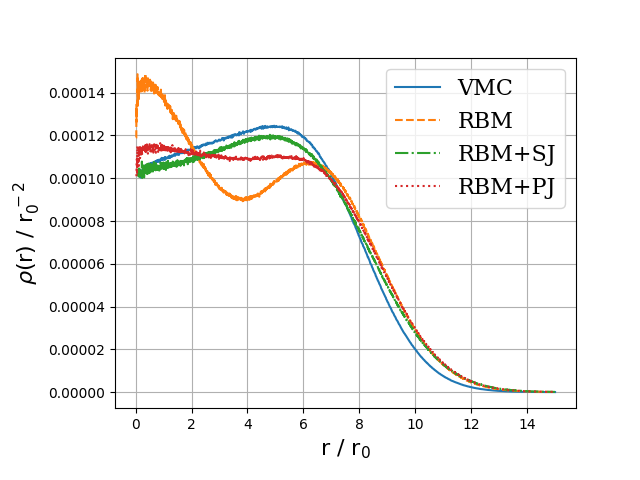
\includegraphics[width=0.9\linewidth]{figures/OB6hw01.png}}

\vspace{6mm}

\end{block}
\end{frame}

\begin{frame}[plain,fragile]
\frametitle{Onebody densities $N=30$, $\hbar\omega=1.0$ a.u.}

\begin{block}{}

\vspace{6mm}

% inline figure
\centerline{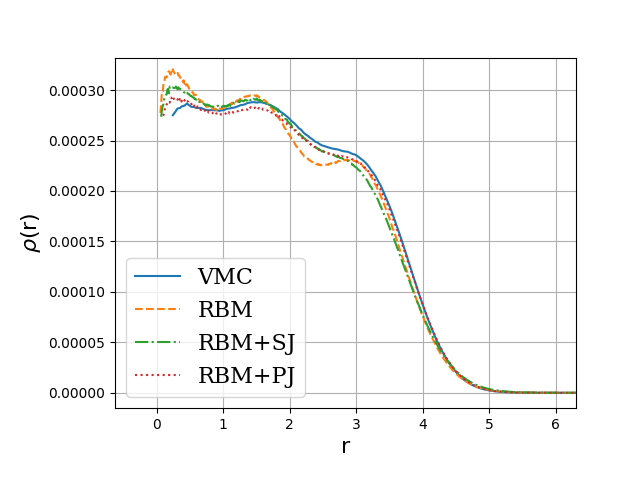
\includegraphics[width=0.9\linewidth]{figures/OB30hw1.png}}

\vspace{6mm}

\end{block}
\end{frame}

\begin{frame}[plain,fragile]
\frametitle{Expectation values as functions of the oscillator frequency}

\begin{block}{}

\vspace{6mm}

% inline figure
\centerline{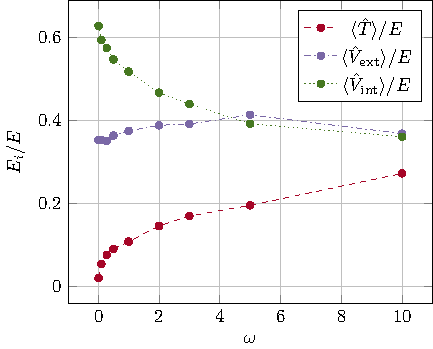
\includegraphics[width=0.9\linewidth]{figures/virialtheorem.pdf}}

\vspace{6mm}

\end{block}
\end{frame}

\begin{frame}[plain,fragile]
\frametitle{Parametric matrix models for rgression type problems}

Given dataset $X\in \mathbb{R}^{n\times m}$, we compute a ``Hamiltonian'' that is linear in the input features $x_i$
\[
\begin{aligned}
        H(X) = \underline{H_0} +\sum_i^mx_i\underline{H_i},
\end{aligned}
\]
Where $H_i\in \mathbb{C}^{N\times N}$.
\end{frame}

\begin{frame}[plain,fragile]
\frametitle{Calcilating eigensystem}

The eigensystem is then calculated for $H$
\[
    H_k = V\Lambda V^\dagger = %
    \begin{bmatrix}
        \vert & \vert & \cdots & \vert \\
        v_1 & v_2 & \cdots & v_{\hyper{l}}\\
        \vert & \vert & \cdots & \vert
    \end{bmatrix}%
    \begin{bmatrix}
        \lambda_1 & & & \\
        & \lambda_2 & & \\
        & & \ddots & \\
        & & & \lambda_{\hyper{l}}
    \end{bmatrix}%
    \begin{bmatrix}
        \vert & \vert & \cdots & \vert \\
        v_1 & v_2 & \cdots & v_{\hyper{l}}\\
        \vert & \vert & \cdots & \vert
    \end{bmatrix}^\dagger
\]
\end{frame}

\begin{frame}[plain,fragile]
\frametitle{Ordering eigenpairs}

Ordering the eigenpairs by decreasing eigenvalue magnitude, $\abs{\lambda^{(k)}_1}\geq\abs{\lambda^{(k)}_2}\geq\cdots\geq\abs{\lambda^{(k)}_l}$, we select the first $\hyper{d}$ eigenvectors to ``decode'' into the penultimate output vector $\vec{z}\in\R^c$,
\[
    z_k = \underline{b_k} + \sum_{i\leq j}^{\hyper{d}}\abs{\vec{v}_i^\dagger \underline{\Delta_{kij}} \vec{v}_j}^2 - \frac{1}{2}\norm{\underline{\Delta_{kij}}}_2^2,
\]
where $\underline{\Delta_{kij}}\in\Herm\left(\hyper{l}\right)$ are trainable Hermitian ``decoder'' matrices and $\underline{\vec{b}}\in\R^c$ is a trainable bias vector. The trainable parameters are trained by minimizing a loss function over all $J$ training points.
\[
    \mathcal{L} = \sum_i\norm{\hat{z}_i-z_i}^P
\]
Where $\hat{z}$ is the true data, and $z$ is the output correspnding to the PMM.
\end{frame}

\end{document}
